

\subsubsection{P0 and mutation count}

A starting point of our experiments was to build a network from P0 data on which to apply modifiers. Select the genes from the communities and then use it to stratify the TCGA tumour the dataset. The hypothesis for this experiment is that to test the power of PGCNA and to stratify the TCGA by the healthy dataset which may yield some interesting results. Thus the following networks are generated for the P0:

% TODO add the meta table
\begin{itemize}
    \item Sizes: 4K-7K
    \item For each size: standard, beta, norm3 and norm2
    \item For each size: 50 edges per Transcription Factor, 3 edges per normal gene
\end{itemize}


% Reason 1 for why this approach is not good - bad gene selection
In the first experiment run, with 4K genes I have noticed that there were not that many changes between communities when the modifier is applied. This is different from what I intended to see when modifiers are applied. We want to see better separation between communities, with smaller and more dedicated biological processes. Thus, I have started investigating this during which I found out that there is a poor representation of the genes mutated in the P0 samples. Thus lead to further investigating on how to select the genes for the PGCNA; this was covered in this section \ref{Sec:N_I:gene_sel}.

To support this argument the following figures are needed:
\begin{itemize}
    \item Sankey plot with the community changes
    \item Bar Figure to show the mutation representation in each community in the P0 dataset. Figure \ref{fig:N_I:P0_median}
    \item Show the mutation intensity (i.e. mutation count) evolution when applying different threshold.  Figure \ref{fig:N_I:P0_comp}
    \item The median gene expression of the genes in each community. See Figure \ref{fig:N_I:P0_comp}.
    \item Experiments with 10K and that there is too much noise. The reason for doing this is that I wanted to have more genes from the P0 included in the Tumour dataset
\end{itemize}

% Reason 2 - Scatter biological pathways 
Further on, when we look at the biology of each community we could see that there a lot shared pathways across communities. This include PDGF, CCKR, apoptosis and others. This gives the impression that the approach developed did the contrary from the intended behaviour, instead of isolating the biological processes it scattered through the network. The pathways were discovered through the Gene Ontology tool using PANTHER Pathway option and \textbf{no correction}; the latter because the majority of the genes inputted were \textbf{not} given significant results. This further strengthen our intuition that this approach is not providing the intended results.

Figures I need to support for the above argument:
\begin{itemize}
    \item Pick 2-3 pathways from the ones found and highlight in the network.
    \item Maybe put the Network with annotations?
\end{itemize}

% Reason 3 - Effect of the TF
While performing the biological interpretation, looking at the genes selected by ModCon score, it can be clearly noticed that the TF genes play a major role in the networks. The reason for this is that in this set of experiment we enable 50 edges for each Transcription Factor, thus biasing the network for these genes. Definitely, this parameter have a large impact of ModCon. Therfore, we performed an experiment with a lower number of edges per TF and we found out that there are more communities with fewer communties.
Figure supporting the above:
\begin{itemize}
    \item How many of the genes selected from the ModCon are a TF? Give some stats
    \item The sub-graph where only the ModCon genes are selected for each community; with the size of the TF \ref{fig:N_1:tf_comp}
\end{itemize}

% Reason 4 - Linking to the tumour stratification 
An open problem to the network selection process is how to link back the genes used in a healthy network to tumour stratification. When tried to apply MEV on the genes selected with the P0 + mutations-count there weren't that well represented in the TCGA's dataset with the same number of genes (4K) - ~1/3 of the genes were presented. However, when all the (basic filtered) 13k genes from the tumour dataset were used, there was a better match. Also, when comparing with the other cohorts didn't make sense, the Basal split wasn't present in neither of the networks. Regardless of the representation, this approach is not fulfilling the initial task which is to integrated the tumour and healthy as it stratifies just by the GE from P0 and doesn't consider the GE from tumour dataset.
To support this argument the following figures are needed:
\begin{itemize}
    \item Stats showing the representation of the selected genes through P0 in the TCGA data
    \item A Morpheus plot with the hierarchical clustering for the one of the P0 experiments
    \item Sankey plot of the Tumour stratification when the genes selected with the P0.
\end{itemize}


\paragraph{Conclusions}

There are a few argument made against this experiment:
\begin{itemize}
    \item The number of connections a gene has a similar effect to the reward modifier. (thinking of the Sankey plot when TF=10 and std-norm3 on P0). This is somehow expected as in the PGCNA paper the author says that more connections yield less communities.
    \item P0 dataset may not have enough power to form smaller communities. This would be verified in the next experiments with TF=10
    \item Many genes from the P0 selection network are missed in the TCGA and the GE of the tumour are not considered.
    \item There is a bias in the gene selection, when the most varied are used, and sometimes the one with the highest magnitude are omitted. Thus experiments to include genes with highest variance, magnitude and mutation count
\end{itemize}


\paragraph{Draft Figures}

\begin{figure}[H]
    \captionsetup[subfigure]{justification=Centering}
    \begin{subfigure}[t]{0.5\textwidth}
        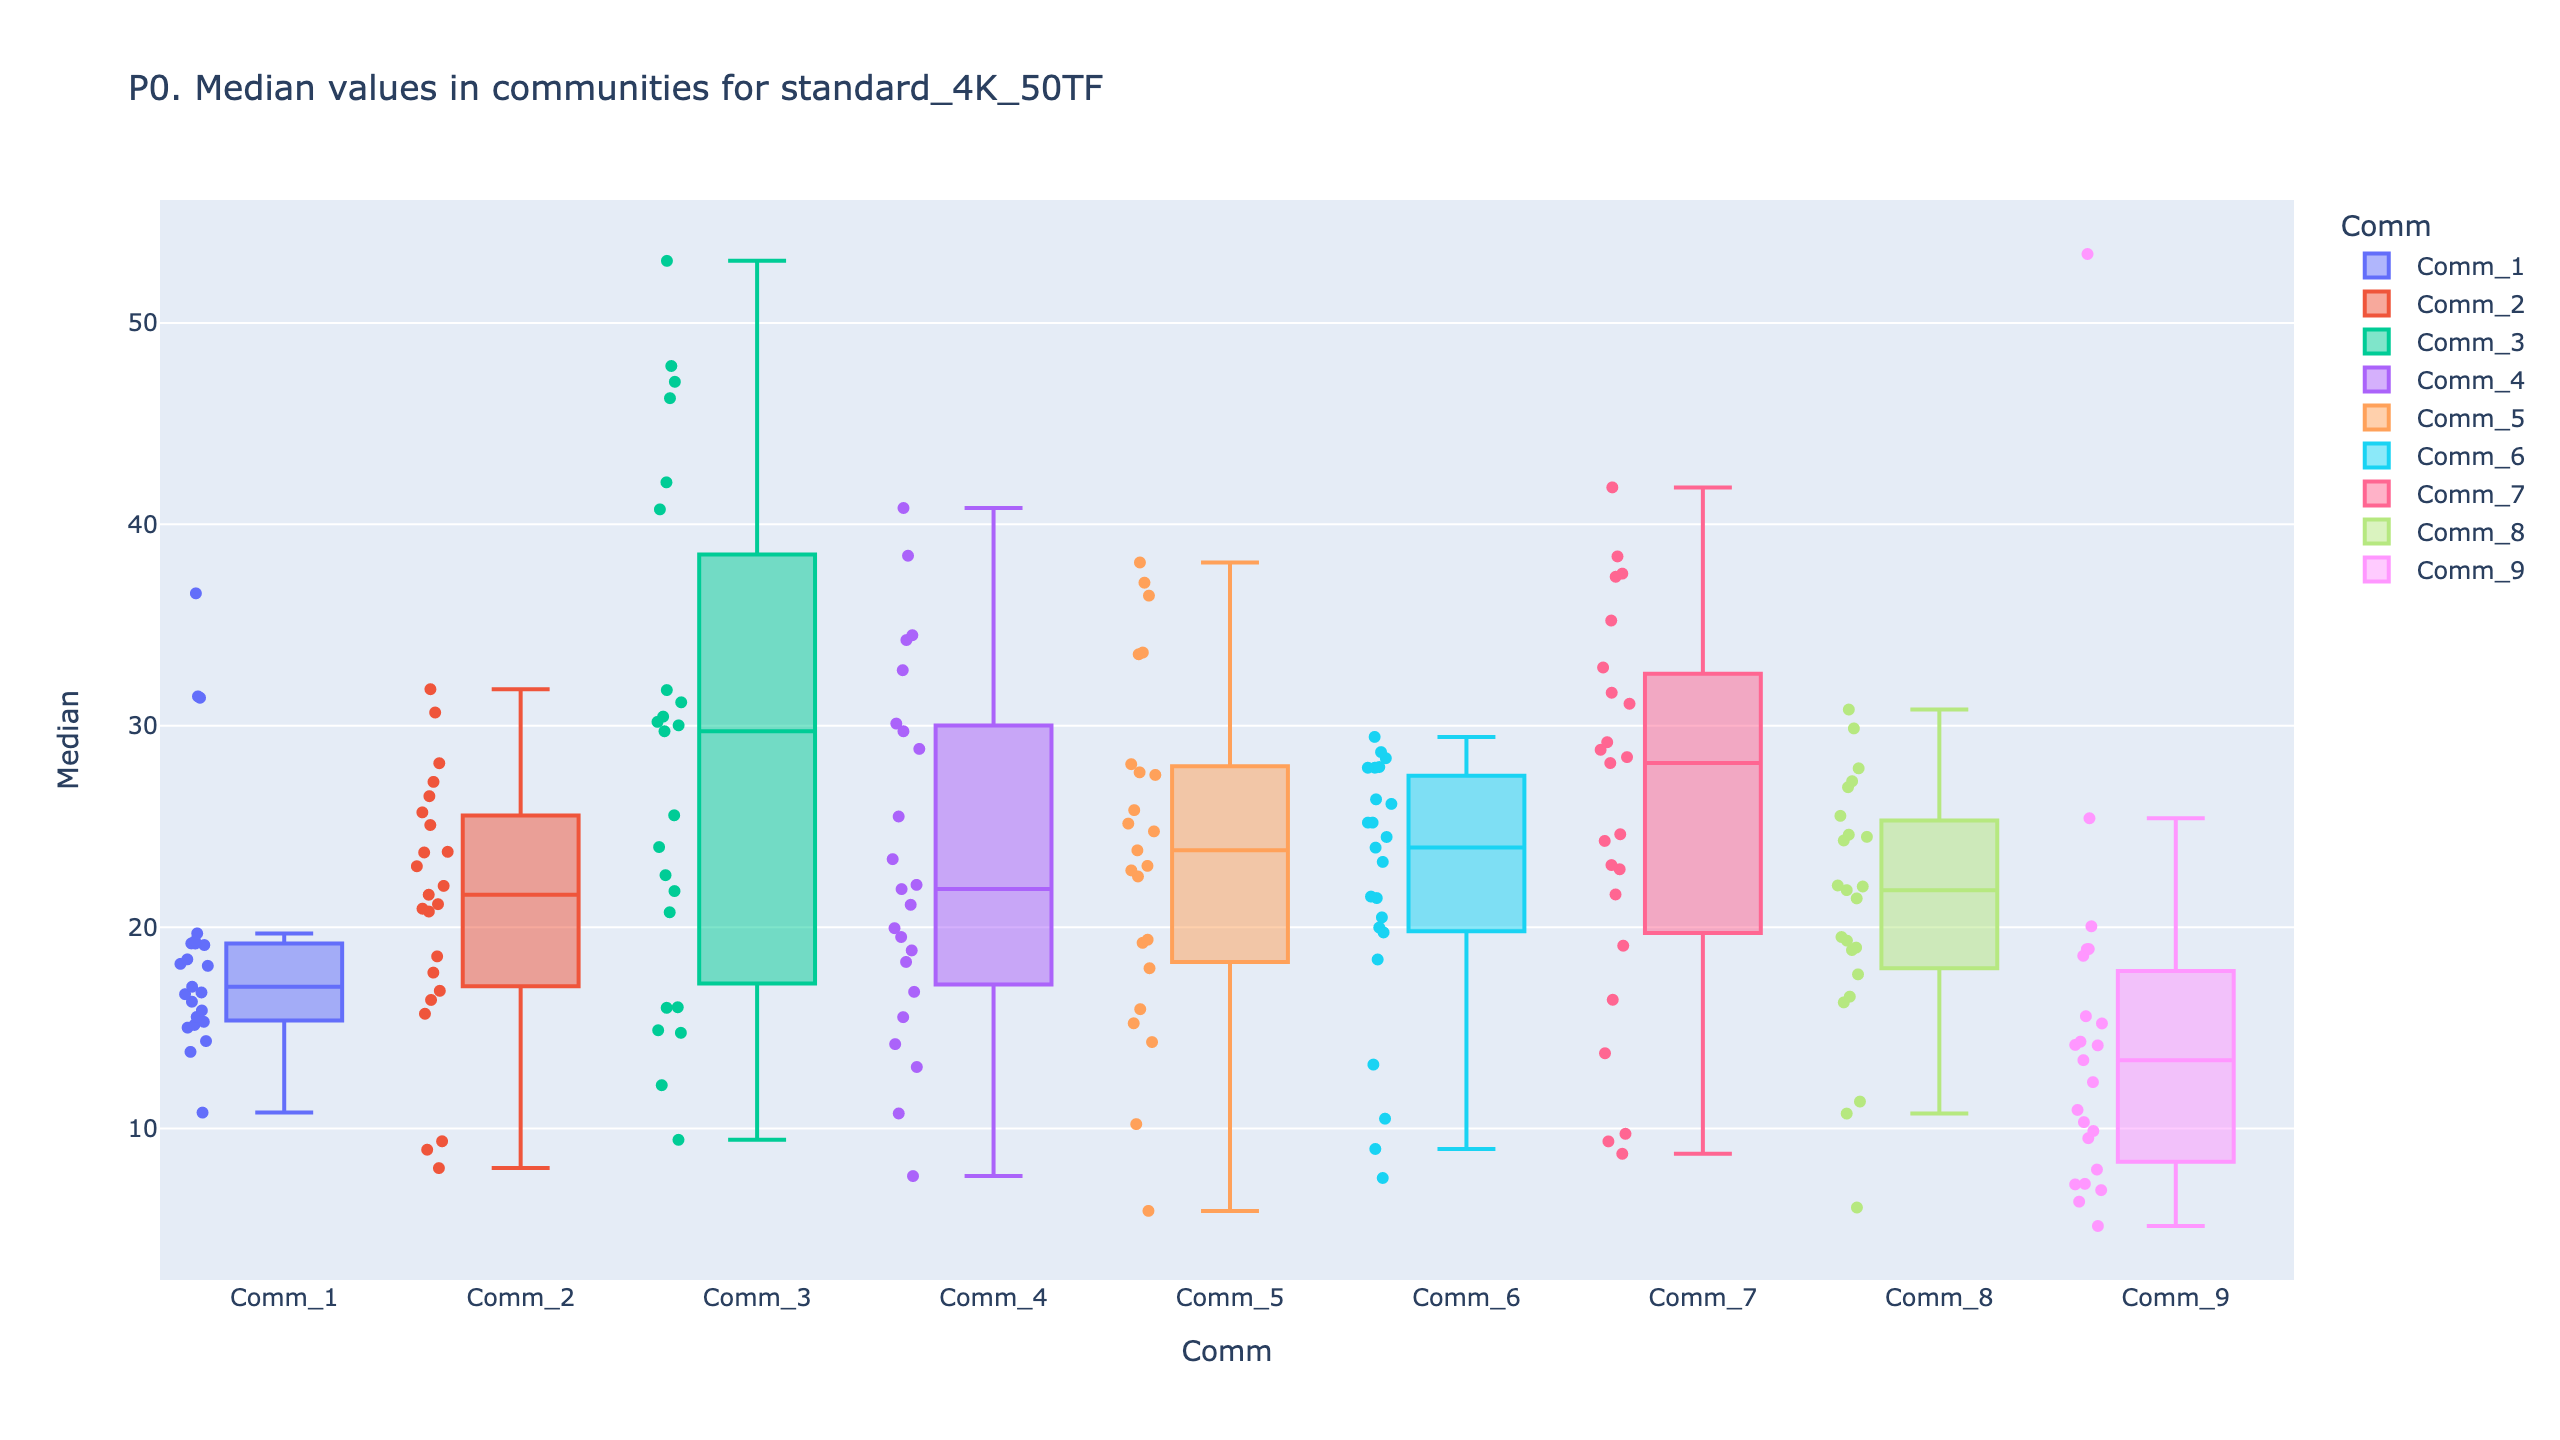
\includegraphics[width=\textwidth]{Images/P0/standard_4K_50TF_median.png}
        \caption{Standard median values}
    \end{subfigure}\hspace{\fill} % maximize horizontal separation
    \bigskip % more vertical separation
    \begin{subfigure}[t]{0.5\textwidth}
        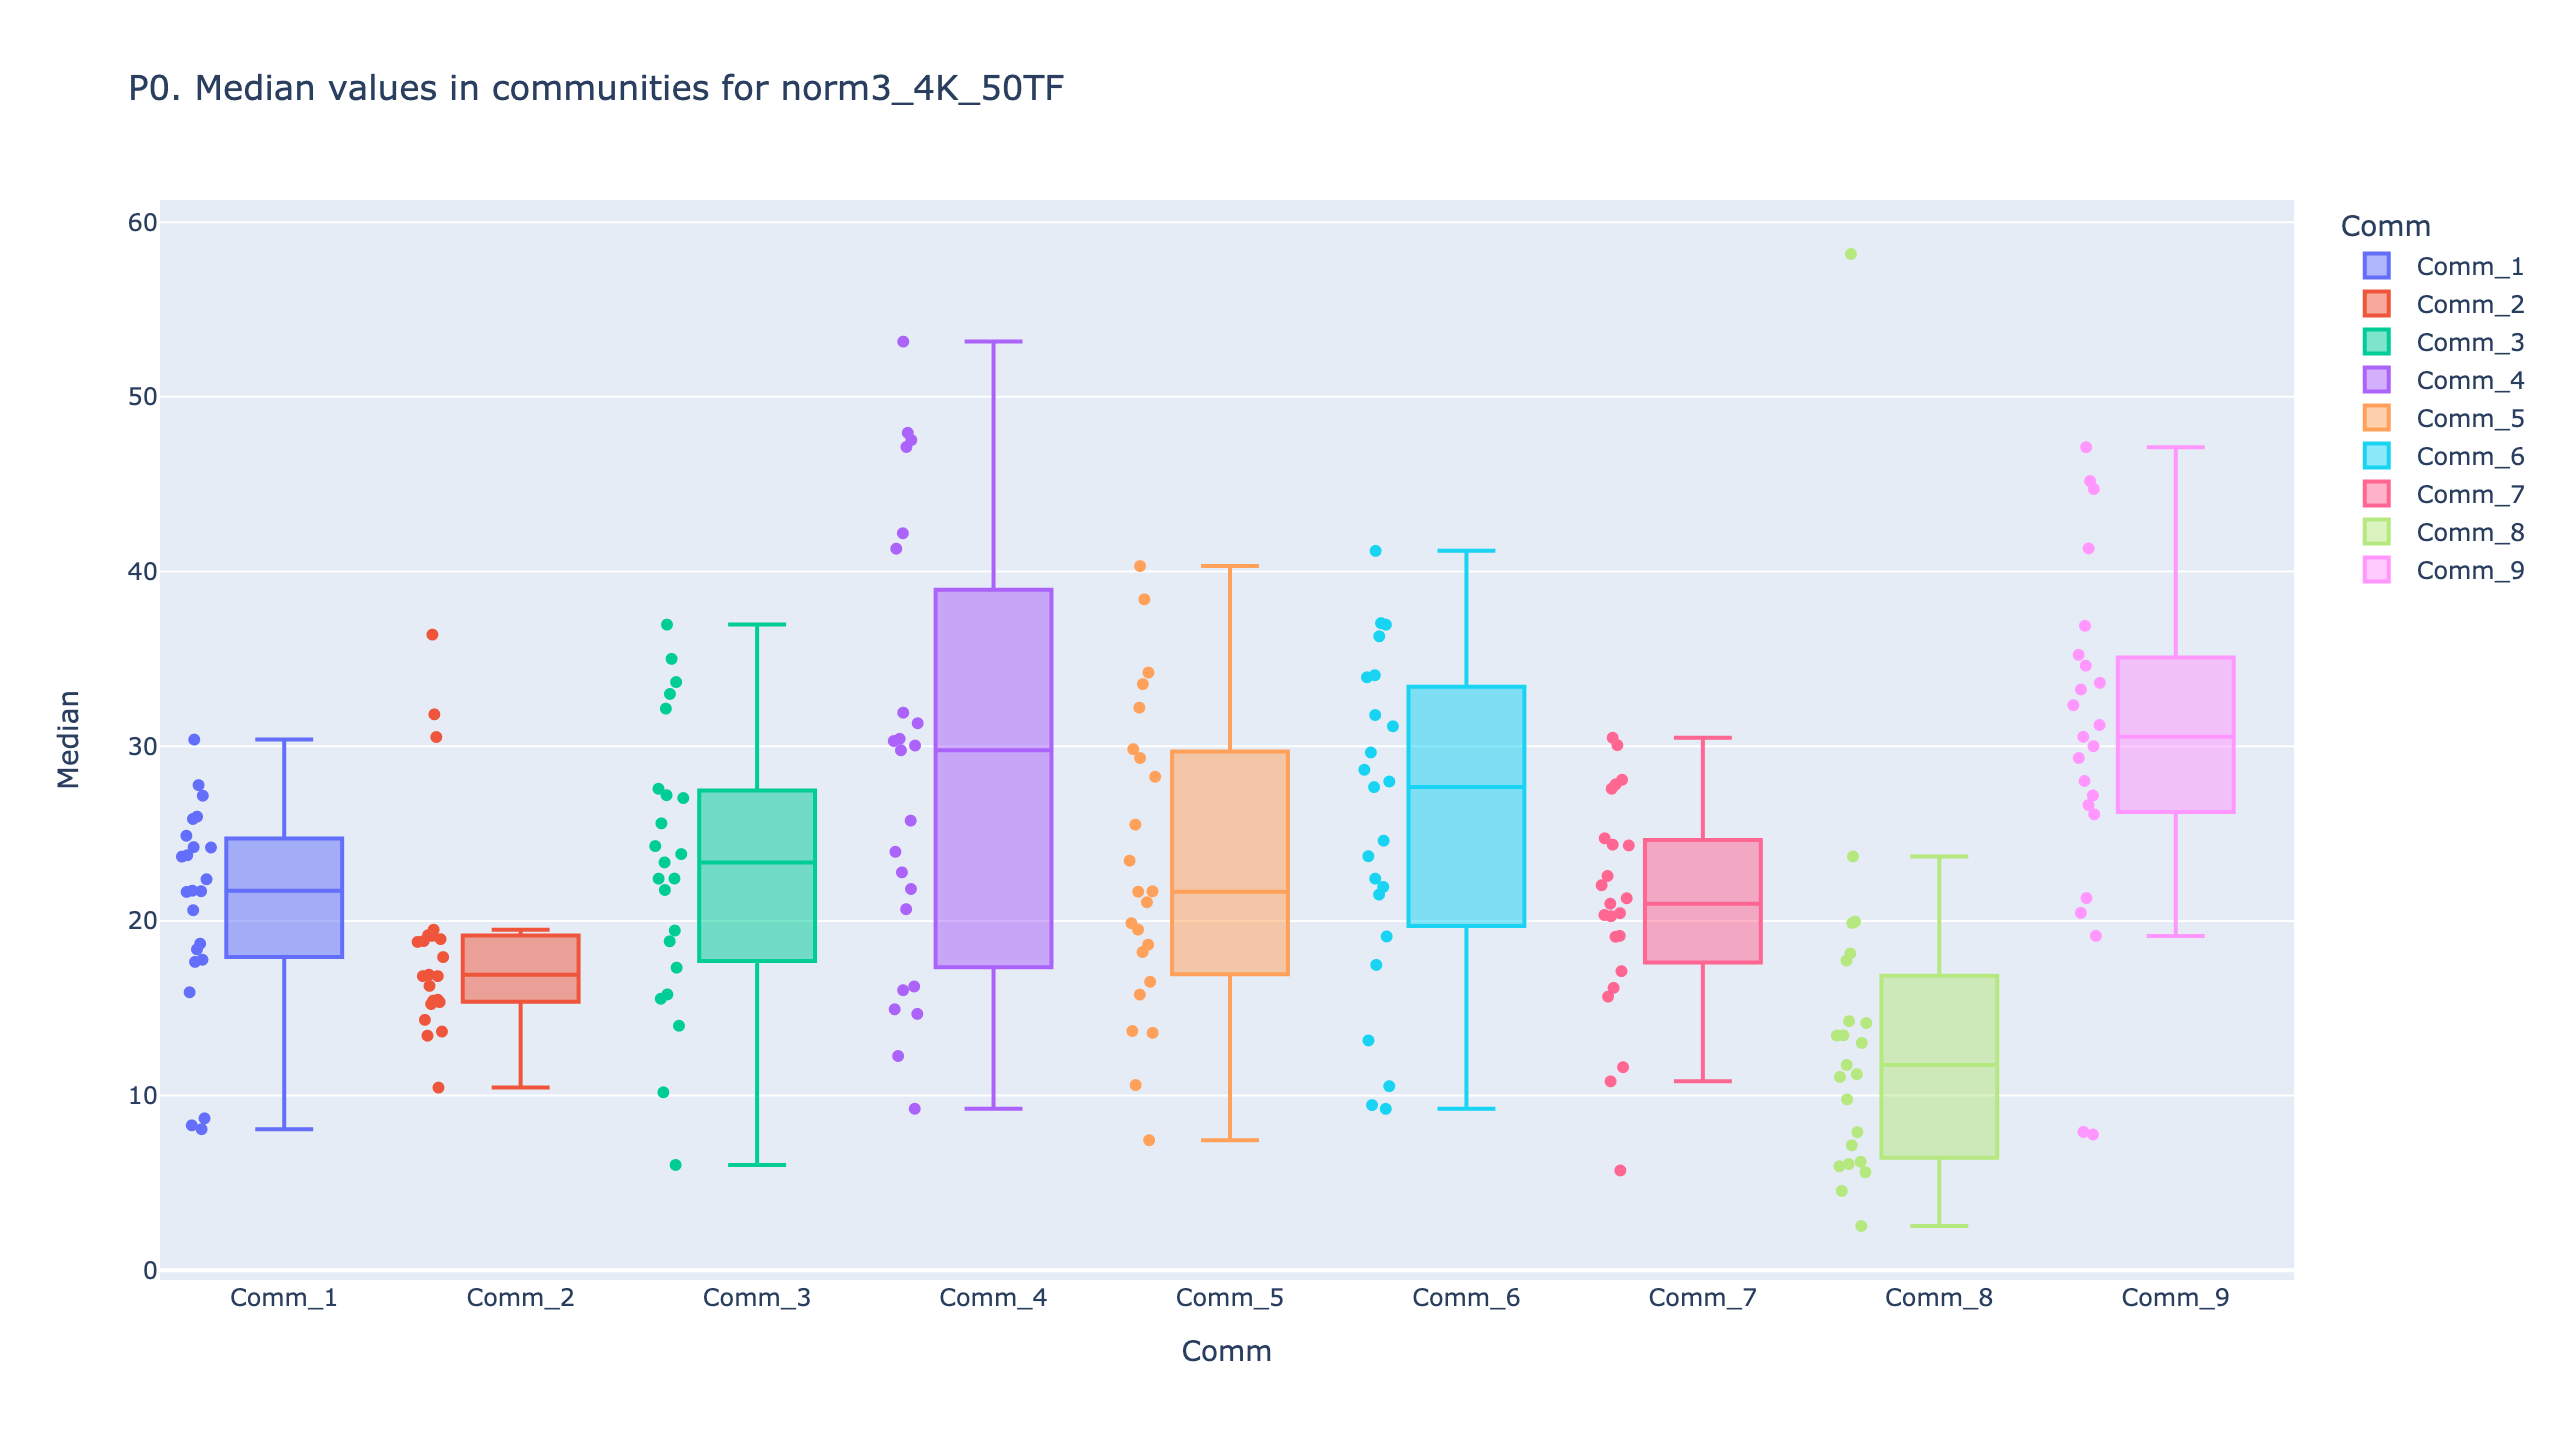
\includegraphics[width=\linewidth]{Images/P0/norm3_4K_50TF_median.png}
        \caption{Norm3 median values}
    \end{subfigure}\hspace{\fill} % maximize horizontal separation
    \caption{Median values for source and target}
    \label{fig:N_I:P0_median}
\end{figure}


\begin{figure}
    \captionsetup[subfigure]{justification=Centering}
    \begin{subfigure}[t]{0.5\textwidth}
        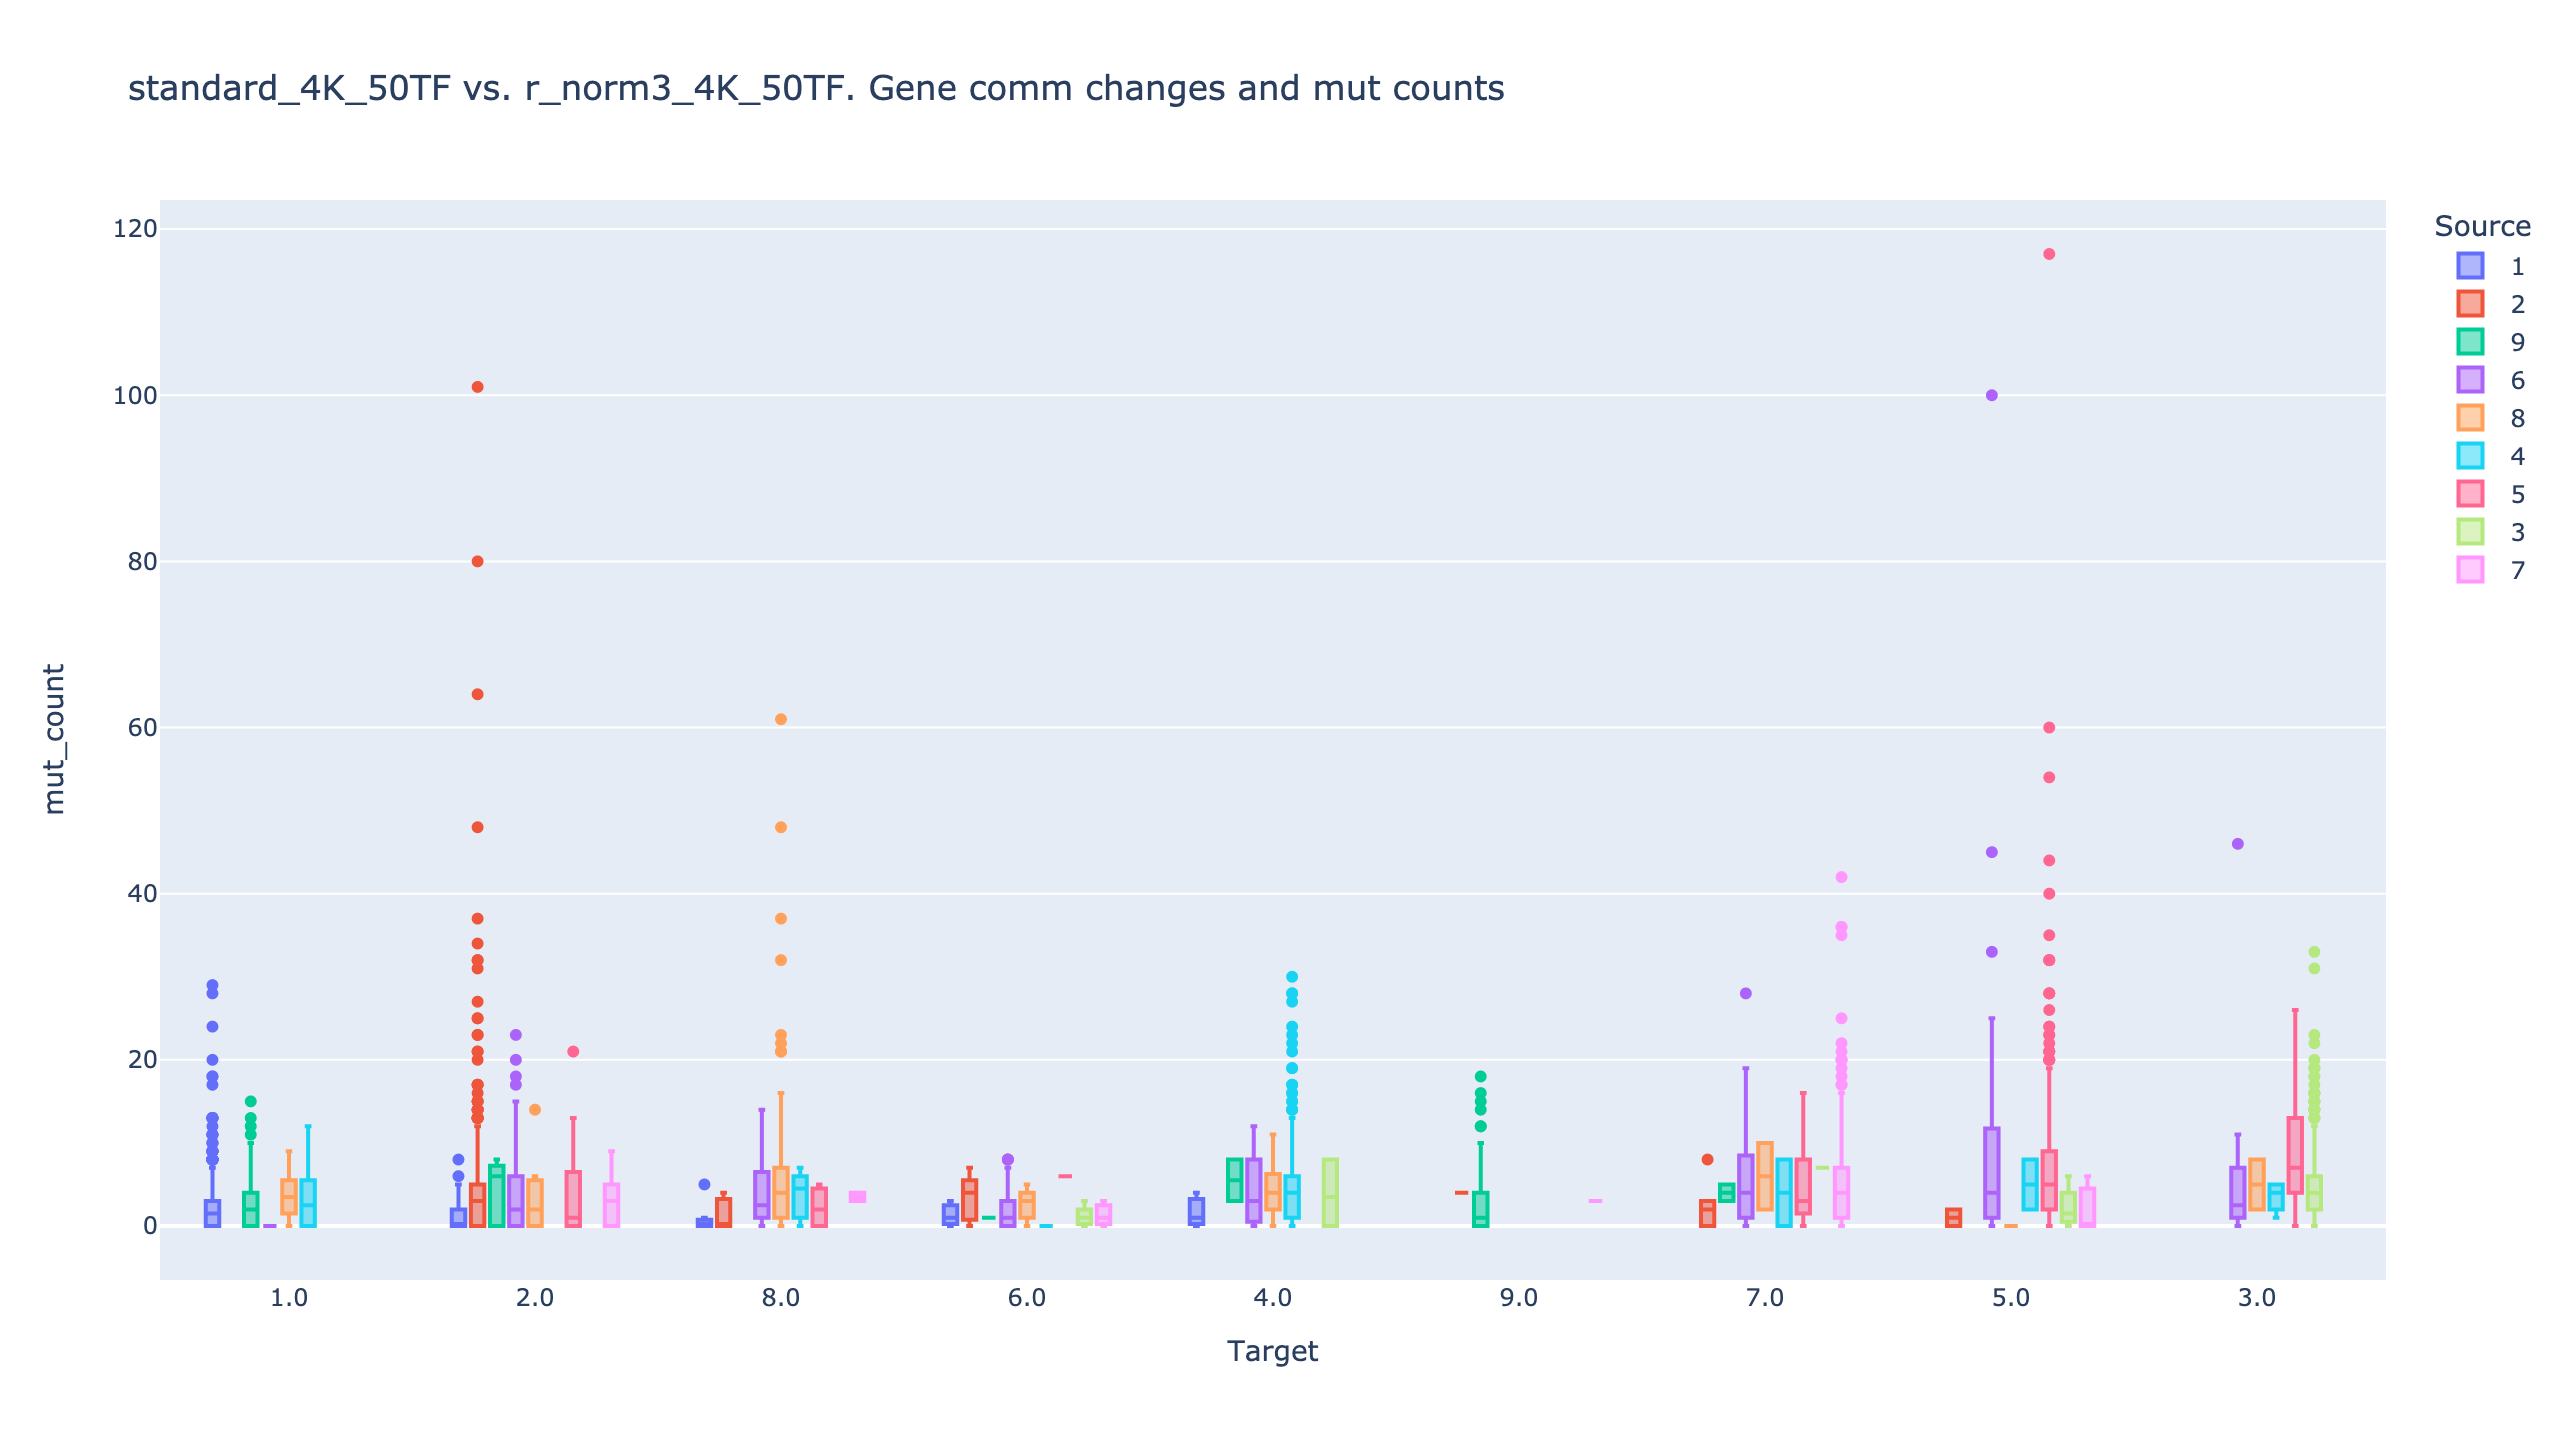
\includegraphics[width=\textwidth]{Images/P0/box_standard_4K_50TF_norm3_4K_50TF.png}
        \caption{Mutation count per community}
    \end{subfigure}\hspace{\fill} % maximize horizontal separation
    \begin{subfigure}[t]{0.5\textwidth}
        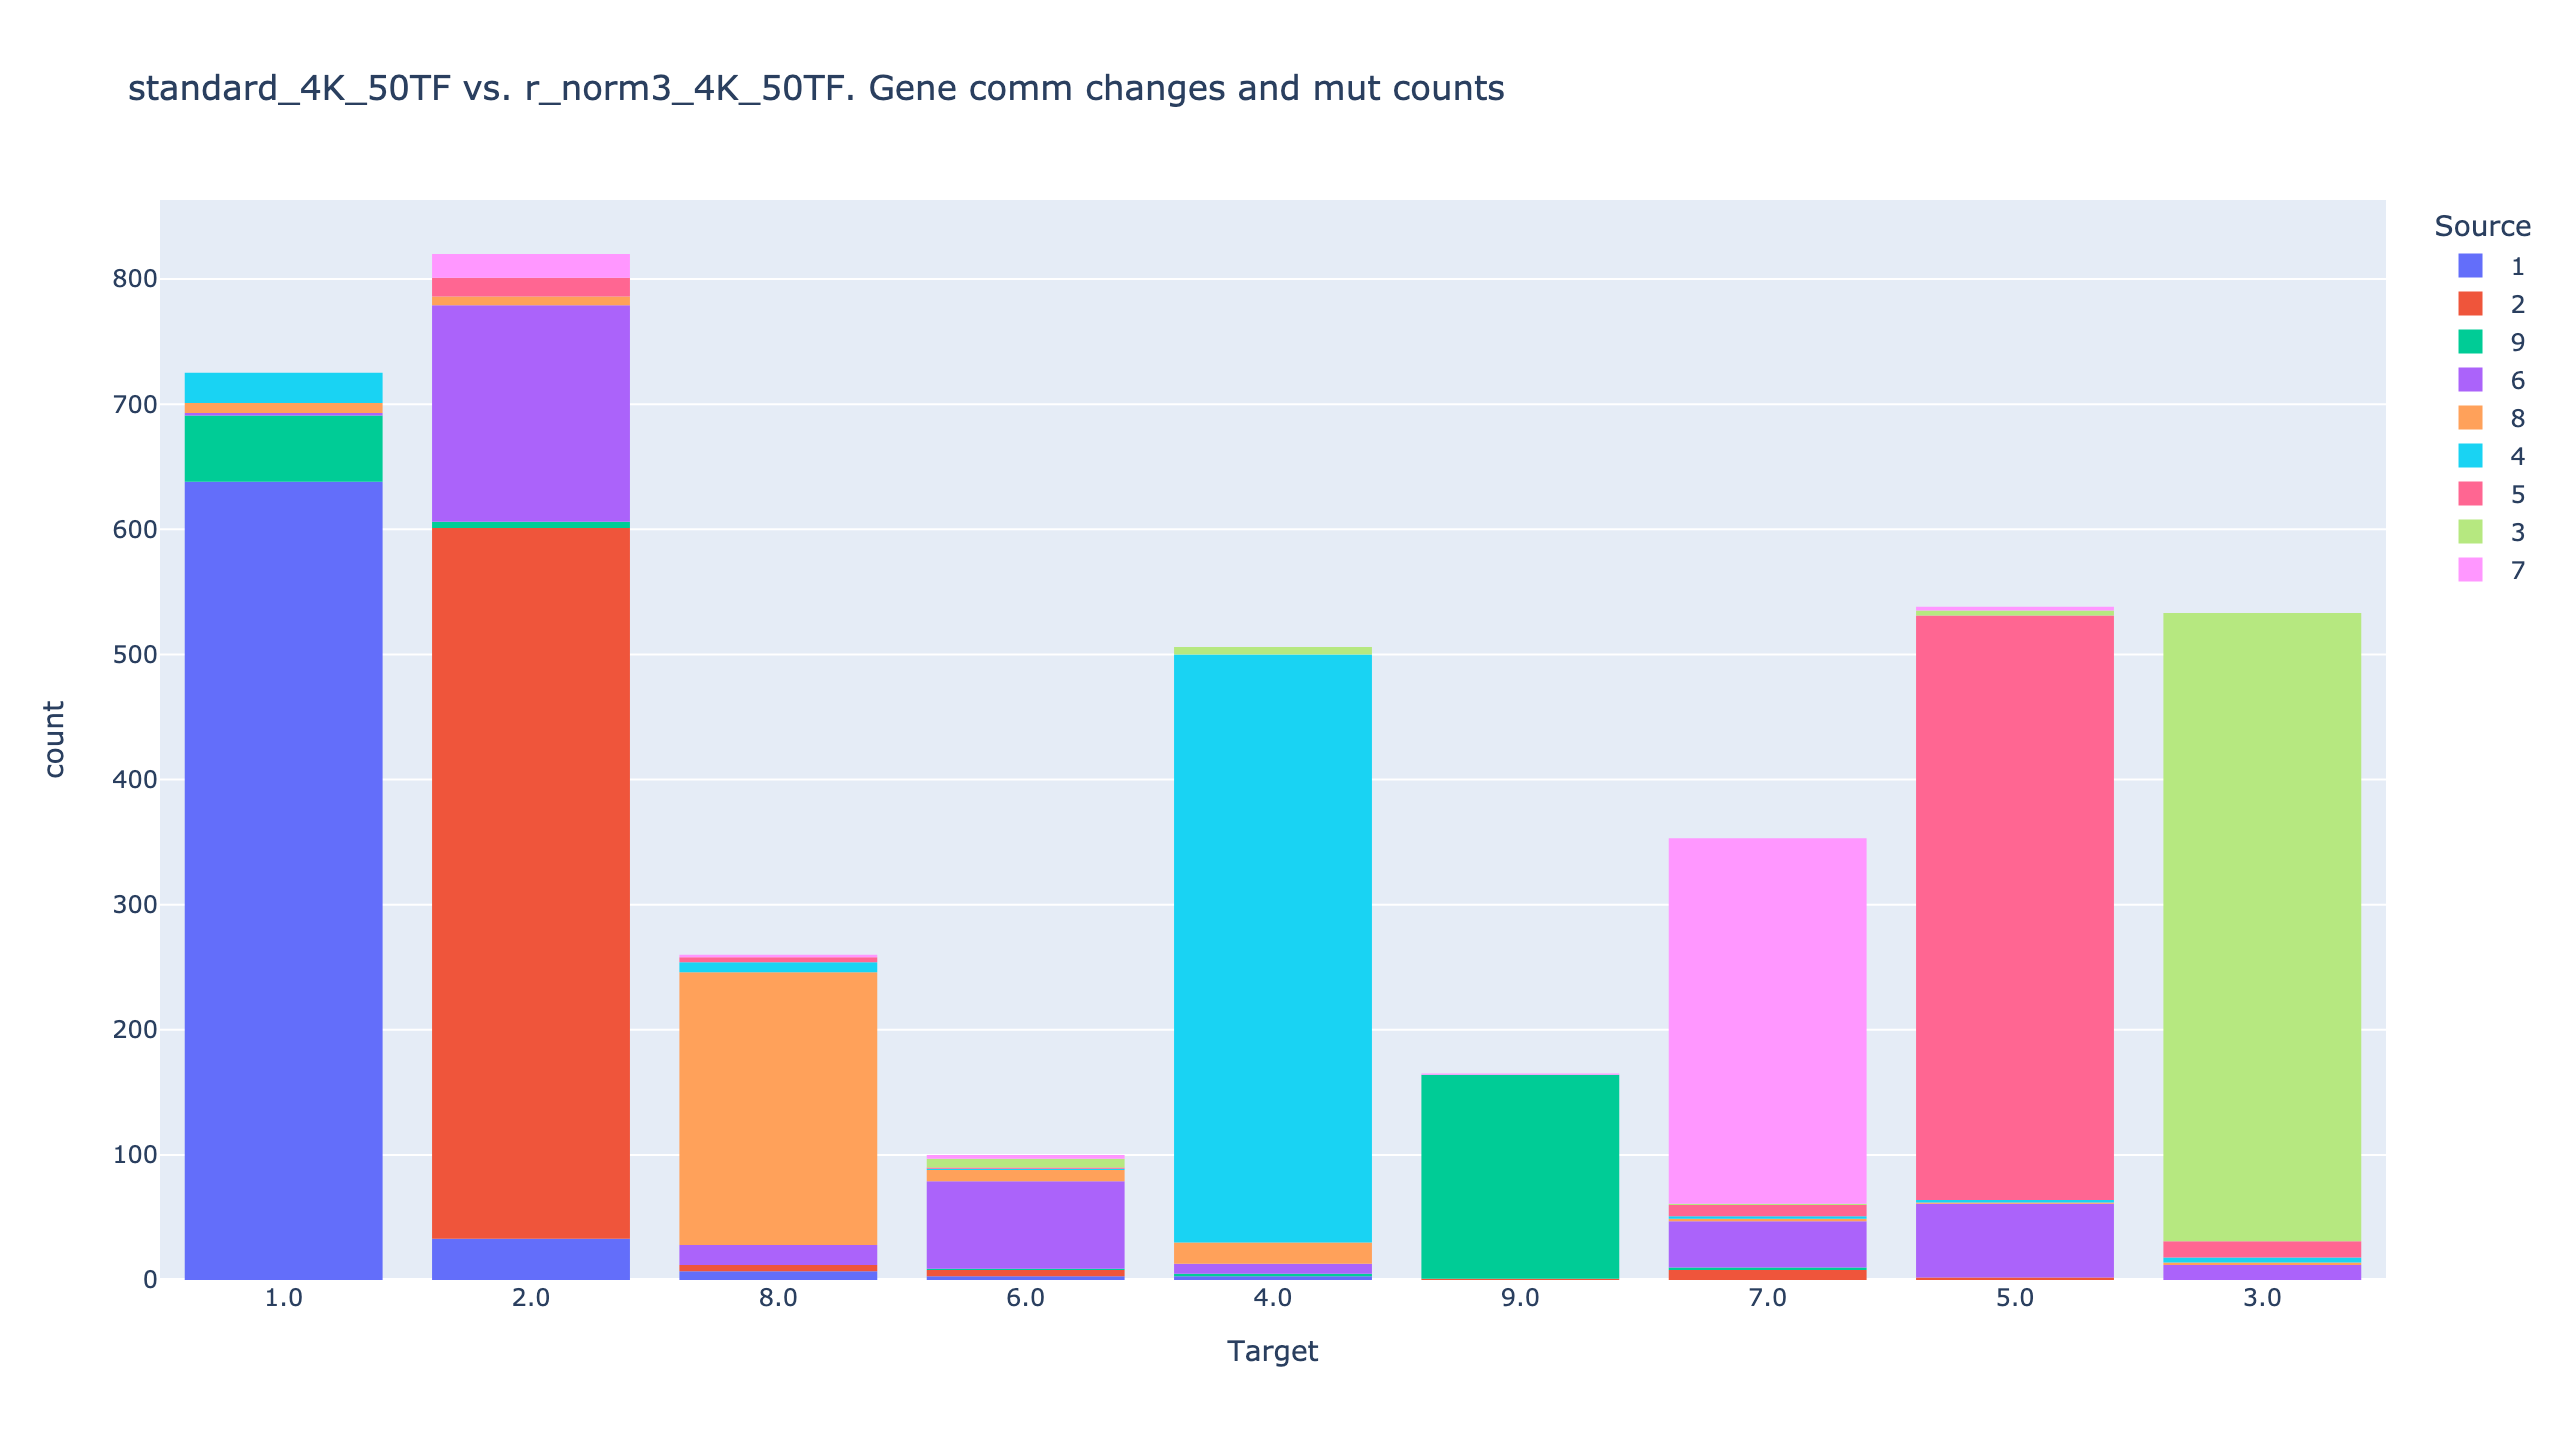
\includegraphics[width=\linewidth]{Images/P0/memberShip_standard_4K_50TF_norm3_4K_50TF.png}
        \caption{Membership changes}
    \end{subfigure}\hspace{\fill} % maximize horizontal separation
    \bigskip % more vertical separation
    \begin{subfigure}[t]{0.9\textwidth}
        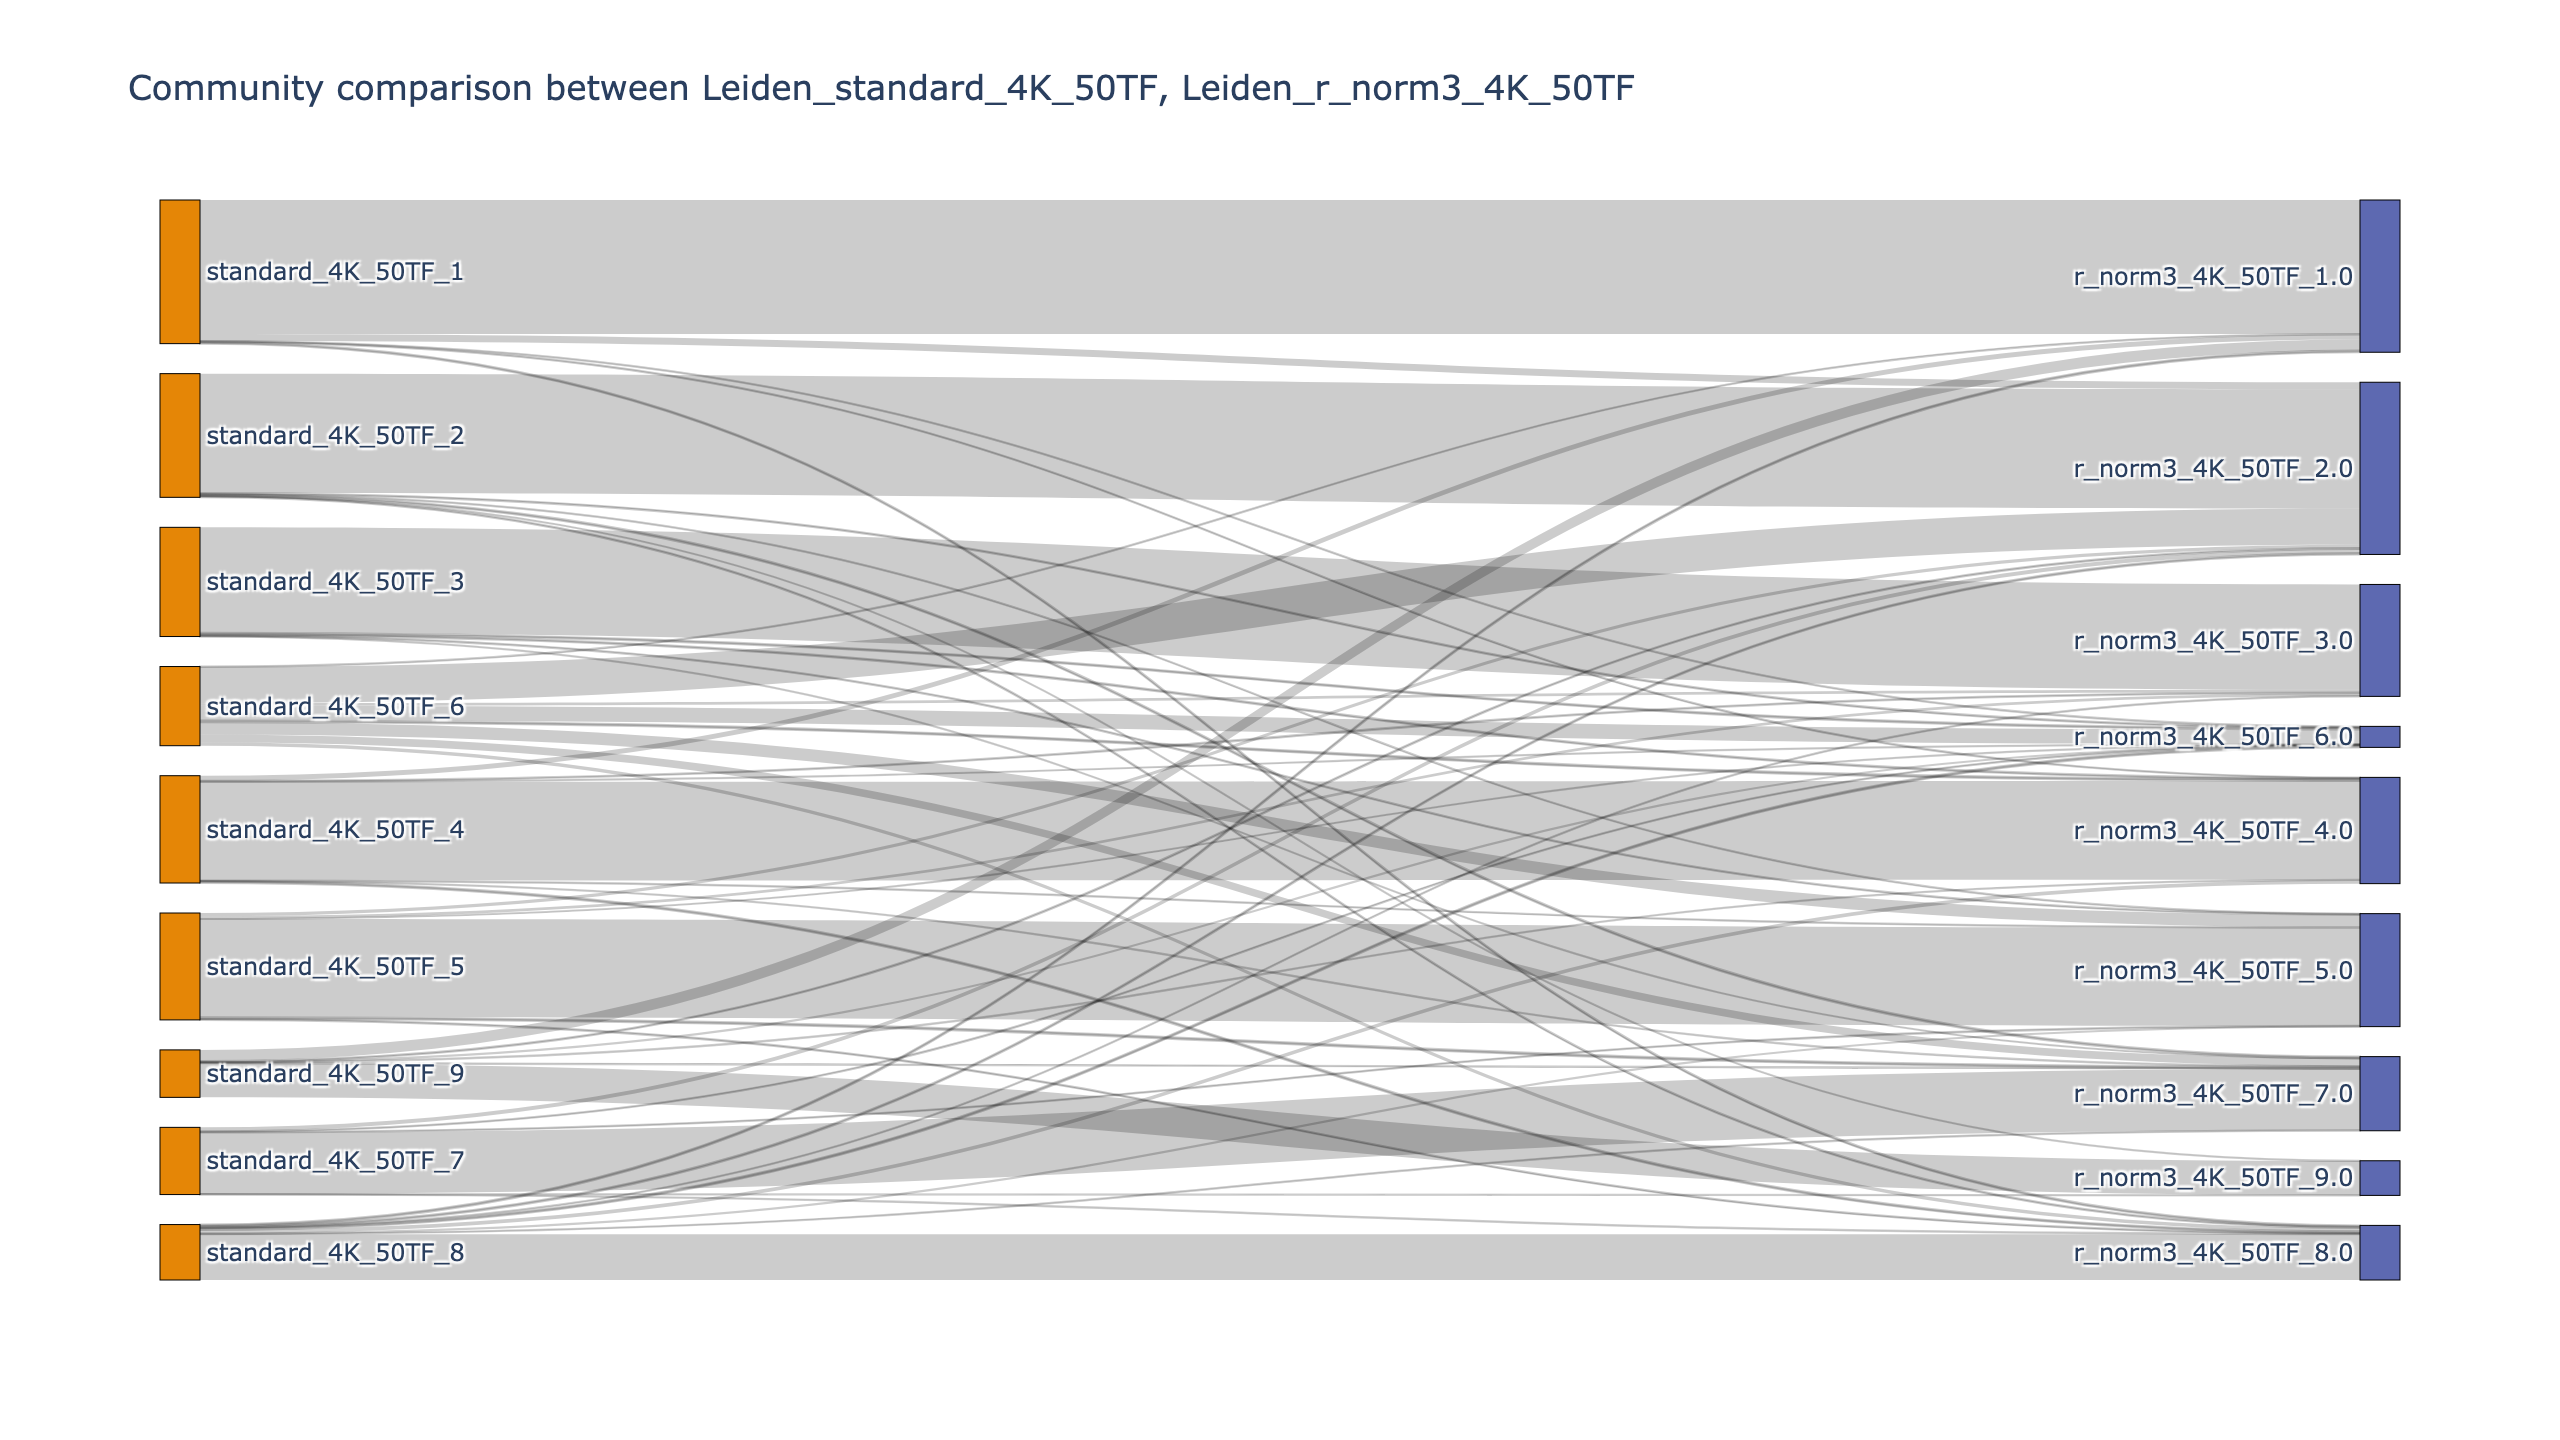
\includegraphics[width=\linewidth]{Images/P0/sankey_standard_4K_50TF_norm3_4K_50TF.png}
        \caption{Sankey between standard and norm3}
    \end{subfigure}\hspace{\fill} % maximize horizontal separation

    \caption{Comparison between Standard and norm3}
    \label{fig:N_I:P0_comp}
\end{figure}



\begin{figure}[!htb]
    \centering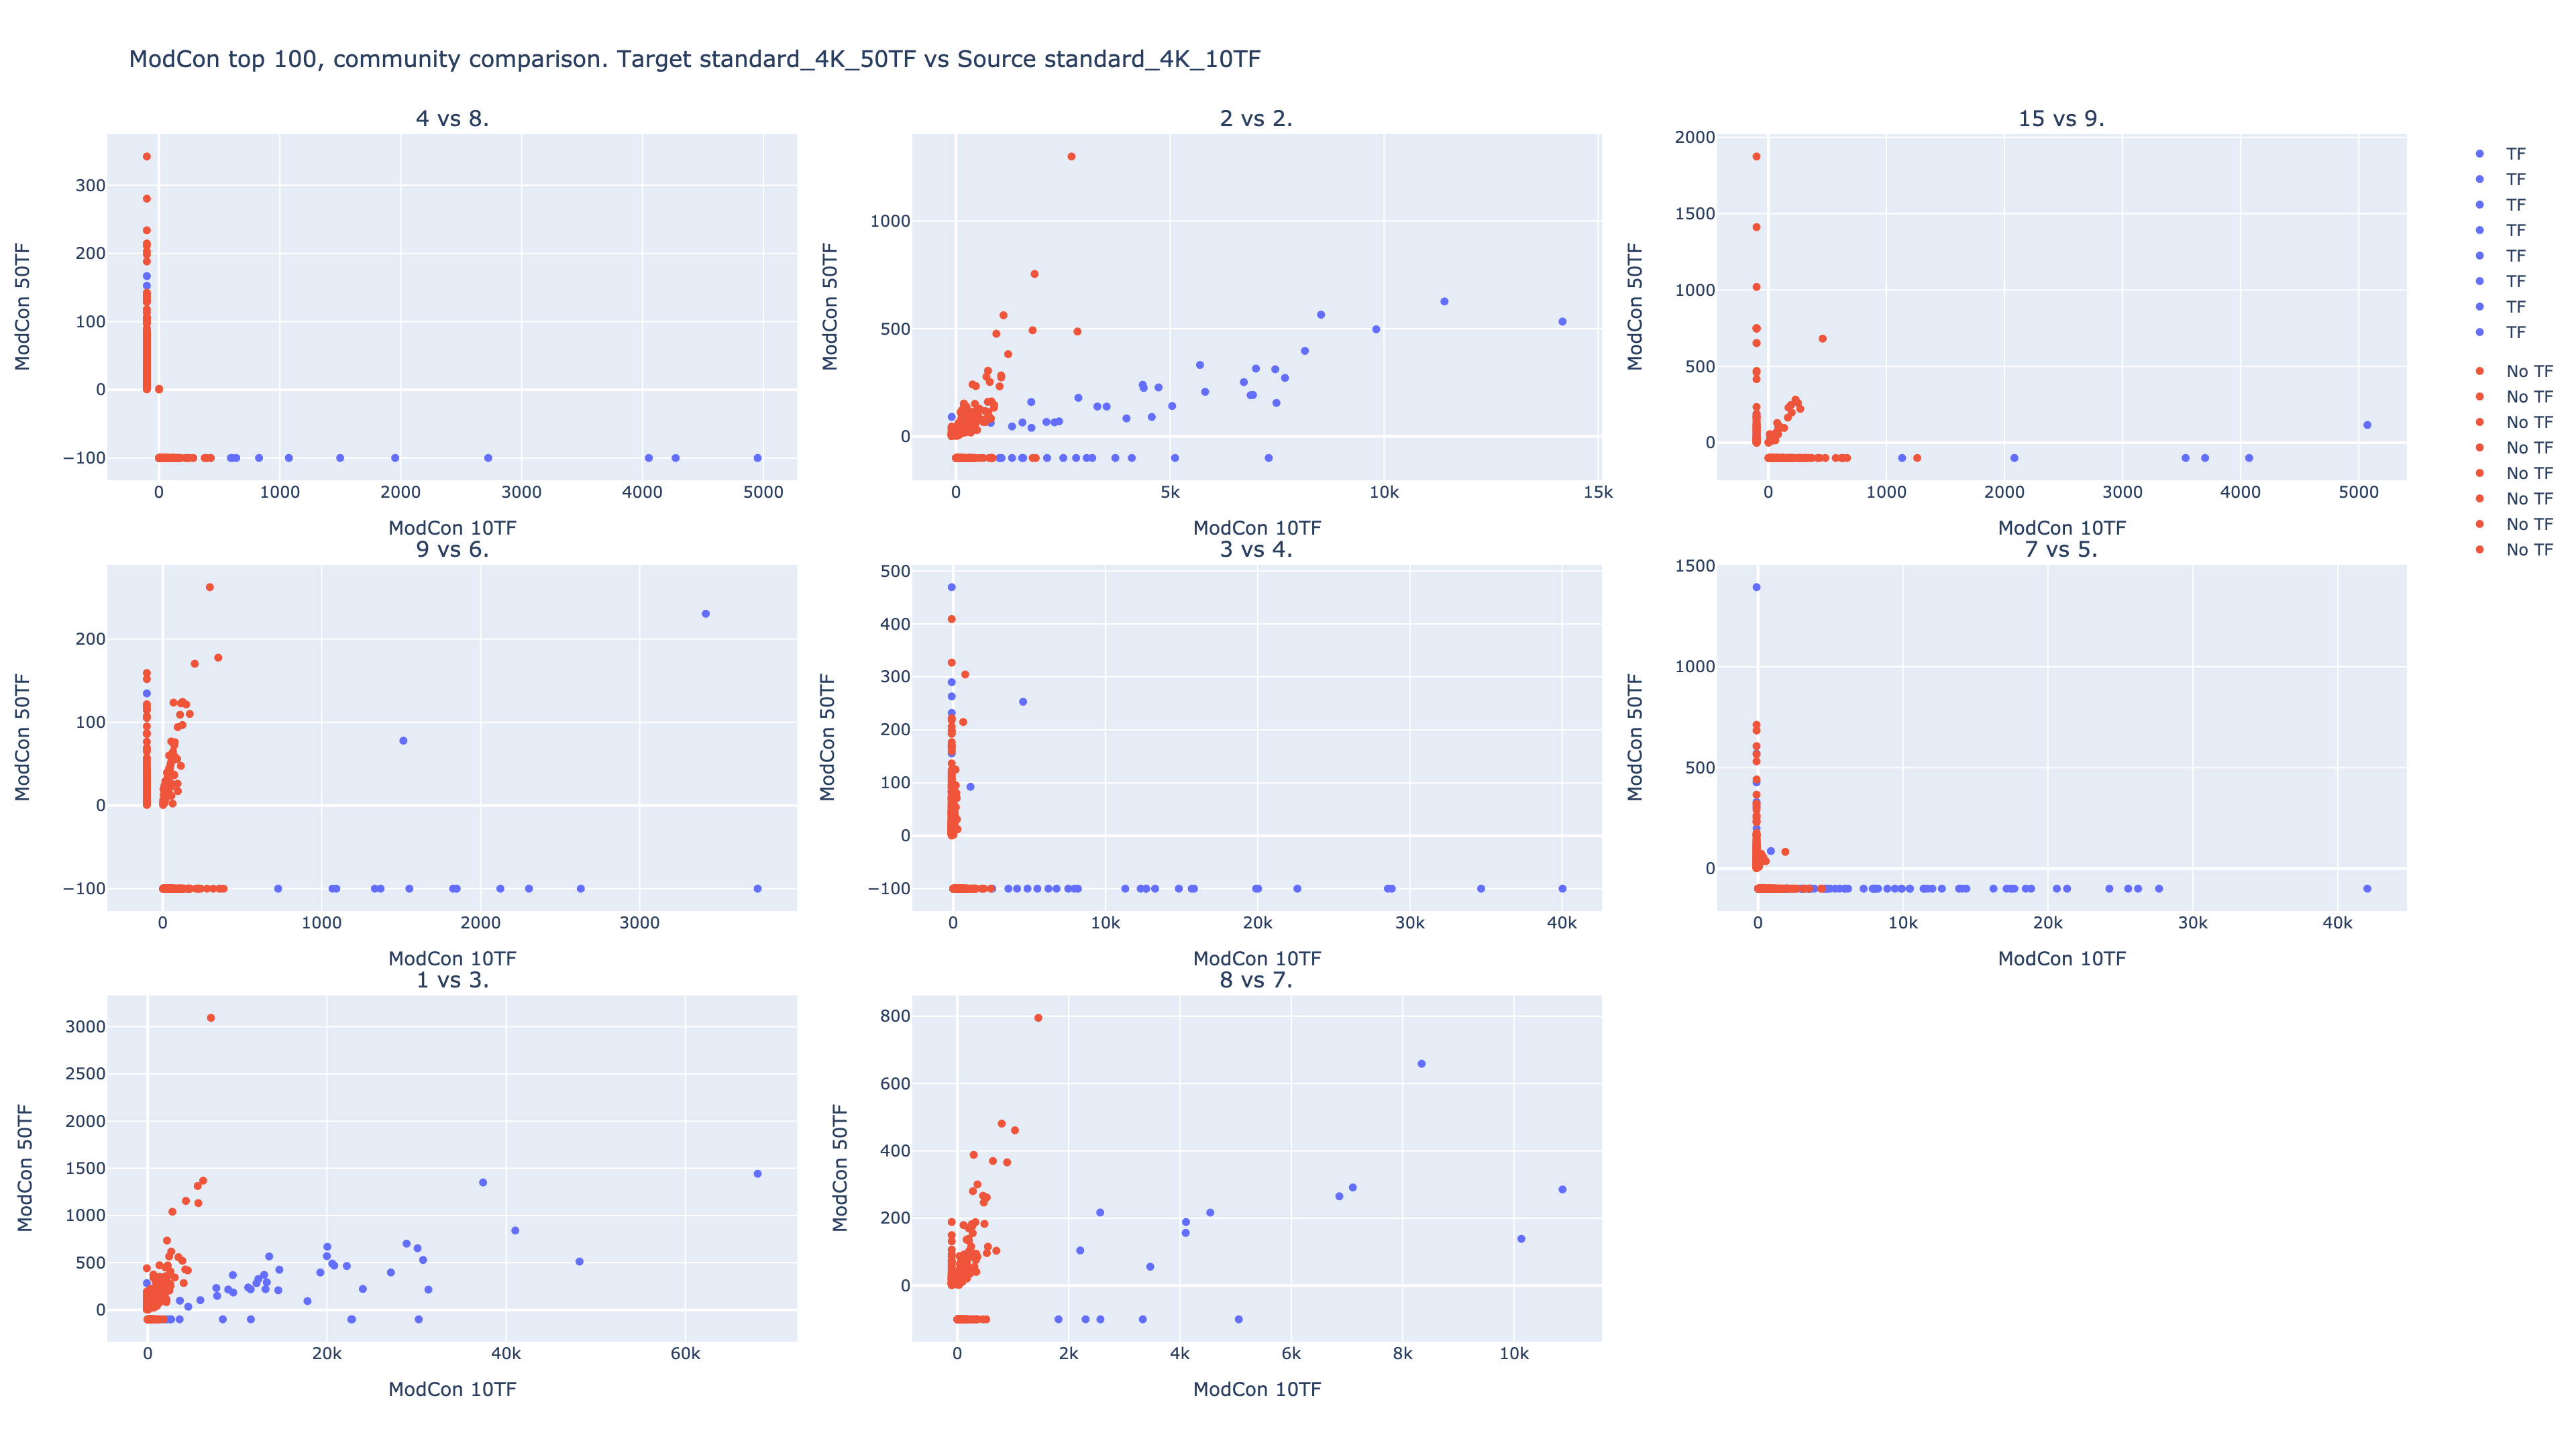
\includegraphics[width=1.0\textwidth,height=1.0\textheight,keepaspectratio]{Images/P0/TF_comp.png}
    \caption{TF Comparison}
    \label{fig:N_1:tf_comp}
\end{figure}

